
\section{Choix}


\begin{frame}
  \frametitle{Choix algorithmiques}

  \begin{block}{Algorithme de Debled et Reveill�s (1995)}
    \begin{itemize}
    \item caract�ristiques $a$, $b$, $\mu$, $\omega$
    \item 4 points d'appui
		\item premier et dernier points
    \item pas de changement d'octant, mais une orientation
    \end{itemize}
  \end{block}

  \begin{exampleblock}{~~~~~~~~~~~~(2,5,0,7)
~~~~~~~~~~~~~~~~~~~~~~~~~~~~~~~~~~~~~~~~~~~~~~~~~~~~~~~~~ (-2,-5,-6,7)}
 \begin{center}
   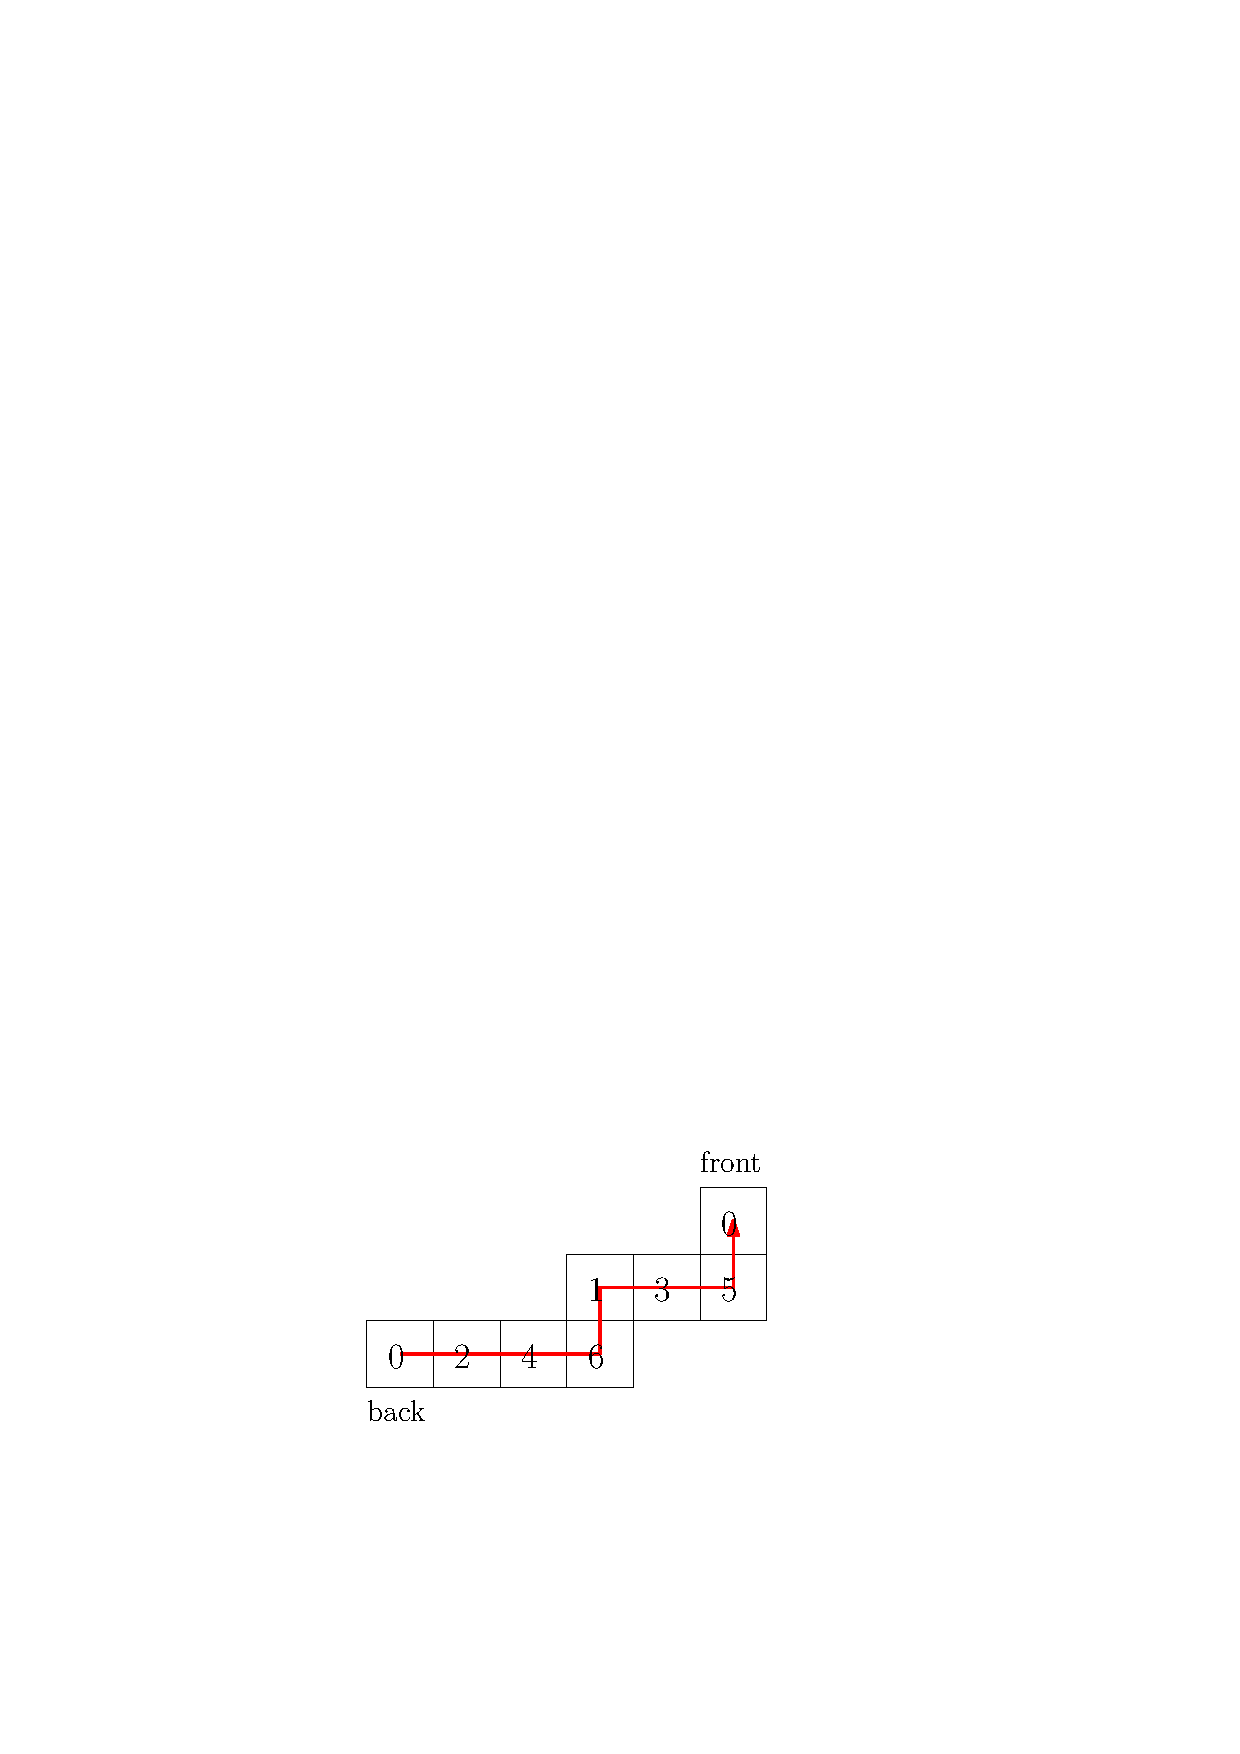
\includegraphics[width=0.3\textwidth,page=1]{DSS}\hspace{0.2\textwidth}
   \includegraphics[width=0.3\textwidth,page=2]{DSS}
 \end{center}
  \end{exampleblock}

\end{frame}

\begin{frame}
  \frametitle{Choix d'impl�mentation}
  

  \begin{block}{Param�tres templates}
    \begin{itemize}
    \item Entier (Domaine ?)
%pas de domaine (image)
    \item Connexit� $\{ \text{na�f}, \text{standard} \}$ 
%eviter les redondances entre les versions
    \end{itemize}
  \end{block}

  \begin{block}{M�thodes principales}
    \begin{itemize}
    \item Initialisation � partir de deux points (un seul point ?)
    \item ajout d'un point � l'avant
		  \begin{itemize}
		  \item \emph{addFront}
			\item prends un point comme param�tre en entr�e (un vecteur, un caract�re ?)
		  \item retourne un booleen (V si DSS, F sinon)
		  \end{itemize}
    \item retrait d'un point � l'arri�re
		  \begin{itemize}
		  \item \emph{removeBack}
			\item pas de param�tre en entr�e
		  \item retourne un booleen (V s'il reste plus de 2 points, F sinon)
		  \end{itemize}
    \end{itemize}
  \end{block}


\end{frame}
